\documentclass[a4paper, 10pt, final]{article}
\usepackage{bonde}

\def\mytitle{Signal and Image Processing 2010}
\def\mysubtitle{Handin of mandatory excercise 5}
\def\myauthor{Ulrik Bonde}
\def\mymail{\mailto{bonde@diku.dk}}
\def\mydate{\today}

\title{\mytitle}
\subtitle{\mysubtitle}

\author{\myauthor{} - \mymail}
\date{\mydate}

\hypersetup{
colorlinks,%
citecolor=black,%
filecolor=black,%
linkcolor=black,%
urlcolor=black,%
bookmarksopen=false,
pdftitle={\mytitle{} - \mysubtitle},
pdfauthor={\myauthor}
}

\begin{document}
\maketitle

\subsection*{Question 5.1}
The following will answer \citep[Excercise 11.6, p. 329]{jahne-digital}.

\paragraph{1)}
I will show that it is not possible to improve the signal-to-noise ratio
for an arbitrary single wave number. The SNR is defined as
\begin{equation}
    SNR = \frac{\sigma^2_N}{\sigma^2_S}
\end{equation}
i.e. the variance of the noise divided by the variance of the signal. By
\citep[Eq. (4.38)]{jahne-digital} we are given a measure for the
variance of a signal convolved with a filter $\mathcal{H}$:
\begin{equation}
    \mathbf{\sigma'} = \sigma^2(\mathcal{H} \star
    \mathcal{H})~ ~\laplace~ ~
    \mathbf{\hat{\sigma}'} = \hat{\sigma}(k)|\hat{\mathcal{H}}|^2
\end{equation}
Using this we write up the SNR for the filtered signal.
\begin{align}
    SNR' & =
    \frac{\sigma^2_N(\mathcal{H}\star\mathcal{H})}{\sigma^2_S(\mathcal{H}\star\mathcal{H})}
    ~ ~\laplace~
    ~\frac{\hat{\sigma}^2_S(k)|\hat{\mathcal{H}}(k)|^2}{\hat{\sigma}^2_N(k)|\hat{\mathcal{H}}(k)|^2}\\
    & = \frac{\sigma^2_N}{\sigma^2_S}
    ~ ~\laplace~
    ~\frac{\hat{\sigma}^2_S(k)}{\hat{\sigma}^2_N(k)}\\
    SNR' & = SNR
\end{align}
The signal to noise ratio is the same in a filtered signal as in the
original signal. Intuitively, if we have a signal and we can divide it
into a signal and noise part, when we filter both parts with the same
filter, then the ratio between the signal and noise will be the same.

\paragraph{2)}
Now, if we assume that we have white noise, but the actual signal only
exist in half of the maximum wave numbers, then we can actually improve
the SNR. The explanation is pretty straight forward. We know in which
frequencies the actual signal is and we know that we have some high
frequency noise. Some of the noise does not interfere with the original
signal, thus we can just remove the frequencies where we \emph{only}
have noise. Fig. \ref{box_filter_model} illustrate this in a two
dimensional signal. The noise is removed by using a box filter.

\begin{figure}[!h]
    \centering
    \subfloat[Original]{\label{org}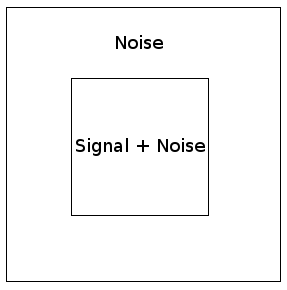
\includegraphics[angle=0,width=0.3\textwidth]{images/spectrum_im_noise}}\hspace{1em}
    \subfloat[Box filter]{\label{box_filter}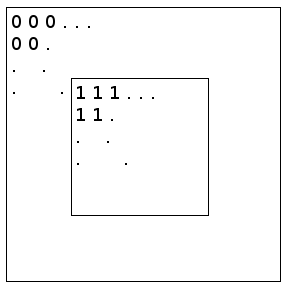
\includegraphics[angle=0,width=0.3\textwidth]{images/filter_box}}\hspace{1em}
    \subfloat[Filtered signal]{\label{filtered}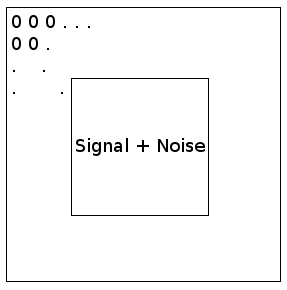
\includegraphics[angle=0,width=0.3\textwidth]{images/filtered_im}}\\
    \caption[]{Frequency representation of the original signal where the
    actual signal is limited to the middle of the power spectrum. Using
    a box filter we can remove the unwanted frequencies, i.e. the noise.
    In the resulting signal these frequencies have been zeroed out.}
    \label{box_filter_model}
\end{figure}

Because we have \emph{only} removed noise and not manipulated the actual
signal we have improved the SNR.

Using an alternative definition for SNR saying
\begin{equation}
    SNR = \frac{\mu}{\sigma_N}
\end{equation}
and realize that $\sigma_N$ is constant (because it is white noise) it
is clear how the SNR is improved. When we remove the unwanted
frequencies the value of $\mu$ is decreased, thus the SNR is improved.

\subsection*{Question 5.2}

%%%%%%%%%%%%%%%%%%%%%%%%%%%%%%%%%%%%%%%%%%%%%%%%%%%%%%%%%%%%%%%%%%%%
% Formal stuff

\bibliographystyle{abbrvnat}
\bibliography{bibliography}
%\addcontentsline{toc}{chapter}{Litteratur}

\appendix
\lstset{language=Matlab, basicstyle=\scriptsize,
    showstringspaces=false, numbers=left, stepnumber=1,
    numberstyle=\tiny, frame=none}
\section{Source code}

\subsection{EdgeDetect.m}
\lstinputlisting{../src/EdgeDetect.m}

\end{document}

% vim: set tw=72 spell spelllang=en:
